\chapter{Developer documentation}

\section{Finite element}

\subsection{Isoparametric element}

$\blacksquare$ Coordinate transformation \cite{XuchengWang2003}

\begin{equation}
{\text{d}} {\bm{\xi}}  = \left[ \begin{gathered}
  \frac{{\partial x}}{{\partial \xi }}{\text{d}}\xi  \hfill \\
  \frac{{\partial y}}{{\partial \xi }}{\text{d}}\xi  \hfill \\
  \frac{{\partial z}}{{\partial \xi }}{\text{d}}\xi  \hfill \\ 
\end{gathered}  \right],{\text{d}} {\bm{\eta}}  = \left[ \begin{gathered}
  \frac{{\partial x}}{{\partial \eta }}{\text{d}}\eta  \hfill \\
  \frac{{\partial y}}{{\partial \eta }}{\text{d}}\eta  \hfill \\
  \frac{{\partial z}}{{\partial \eta }}{\text{d}}\eta  \hfill \\ 
\end{gathered}  \right],{\text{d}} {\bm{\zeta}}  = \left[ \begin{gathered}
  \frac{{\partial x}}{{\partial \zeta }}{\text{d}}\zeta  \hfill \\
  \frac{{\partial y}}{{\partial \zeta }}{\text{d}}\zeta  \hfill \\
  \frac{{\partial z}}{{\partial \zeta }}{\text{d}}\zeta  \hfill \\ 
\end{gathered}  \right]
\end{equation}

Partial derivatives, Jacobian matrix, gradient tensor

\begin{equation}
\left[ {\begin{array}{c}
  {\frac{{\partial {N_i}}}{{\partial \xi }}} \\ 
  {\frac{{\partial {N_i}}}{{\partial \eta }}} \\ 
  {\frac{{\partial {N_i}}}{{\partial \zeta }}} 
\end{array}} \right] = \left[ {\begin{array}{ccc}
  {\frac{{\partial x}}{{\partial \xi }}}&{\frac{{\partial y}}{{\partial \xi }}}&{\frac{{\partial z}}{{\partial \xi }}} \\ 
  {\frac{{\partial x}}{{\partial \eta }}}&{\frac{{\partial y}}{{\partial \eta }}}&{\frac{{\partial z}}{{\partial \eta }}} \\ 
  {\frac{{\partial x}}{{\partial \zeta }}}&{\frac{{\partial x}}{{\partial \zeta }}}&{\frac{{\partial x}}{{\partial \zeta }}} 
\end{array}} \right]\left[ {\begin{array}{c}
  {\frac{{\partial {N_i}}}{{\partial x}}} \\ 
  {\frac{{\partial {N_i}}}{{\partial y}}} \\ 
  {\frac{{\partial {N_i}}}{{\partial z}}} 
\end{array}} \right], { {\bm{J}}^{\text{T}}} = \frac{{\partial \left( {x,y,z} \right)}} {{\partial \left( {\xi ,\eta ,\zeta } \right)}} = {\nabla _{\bm{\xi}} } {\bm{x}}
\end{equation}

\begin{equation}
{{\bm{J}}^T} = \left[ {\begin{array}{cccc}
  {\frac{{\partial {N_1}}}{{\partial \xi }}}&{\frac{{\partial {N_2}}}{{\partial \xi }}}& \cdots &{\frac{{\partial {N_m}}}{{\partial \xi }}} \\ 
  {\frac{{\partial {N_1}}}{{\partial \eta }}}&{\frac{{\partial {N_2}}}{{\partial \eta }}}& \cdots &{\frac{{\partial {N_m}}}{{\partial \eta }}} \\ 
  {\frac{{\partial {N_1}}}{{\partial \zeta }}}&{\frac{{\partial {N_2}}}{{\partial \zeta }}}& \cdots &{\frac{{\partial {N_m}}}{{\partial \zeta }}} 
\end{array}} \right]\left[ {\begin{array}{ccc}
  {{x_1}}&{{y_1}}&{{z_1}} \\ 
  {{x_2}}&{{y_2}}&{{z_2}} \\ 
   \vdots & \vdots & \vdots  \\ 
  {{x_m}}&{{y_m}}&{{z_m}} 
\end{array}} \right]
\end{equation}

Infinitesimal volume

\begin{equation}
{\rm{d}}V = {\rm{d}} {\bm{\xi}}  \cdot \left( {{\rm{d}} {\bm{\eta}}  \times {\rm{d}} {\bm{\zeta}} } \right) = \left| J \right|{\rm{d}}\xi {\rm{d}}\eta {\rm{d}}\zeta 
\end{equation}

Infinitesimal area

\begin{equation}
{\text{d}}A = {\left| {{\text{d}} {\bm{\eta}} \times {\text{d}} {\bm{\zeta}} } \right|_{\xi  = {\text{const}}}} = \sqrt {{{\left( {\frac{{\partial y}}{{\partial \eta }}\frac{{\partial z}}{{\partial \zeta }} - \frac{{\partial y}}{{\partial \zeta }}\frac{{\partial z}}{{\partial \eta }}} \right)}^2} + {{\left( {\frac{{\partial z}}{{\partial \eta }}\frac{{\partial x}}{{\partial \zeta }} - \frac{{\partial z}}{{\partial \zeta }}\frac{{\partial x}}{{\partial \eta }}} \right)}^2} + {{\left( {\frac{{\partial x}}{{\partial \eta }}\frac{{\partial y}}{{\partial \zeta }} - \frac{{\partial x}}{{\partial \zeta }}\frac{{\partial y}}{{\partial \eta }}} \right)}^2}} {\text{d}}\eta {\text{d}}\zeta 
\end{equation}

\subsection{Numerical integration}

$\blacksquare$ Gauss Legendre quadrature over a triangle \cite{RathodHT2004}

From Cartesian coordinate to area/barycentric/natural coordinate

\begin{equation}
\left\{ \begin{gathered}
  x = {L_i}{x_i} + {L_j}{x_j} + {L_m}{x_m} \hfill \\
  y = {L_i}{y_i} + {L_j}{y_j} + {L_m}{y_m} \hfill \\ 
\end{gathered}  \right.
\end{equation}

\begin{equation}
{\text{d}}{x}{\text{d}}{y} = 2A{\text{d}}{L_i}{\text{d}}{L_j}
\end{equation}
where $A$ is the area of the triangle and is constant.

From triangle to standard triangle as shown in Fig.~\ref{fig:tfst}

\begin{equation}
\left\{ \begin{gathered}
  {L_i} = s \hfill \\
  {L_j} = t \hfill \\
  {L_m} = 1 - s - t \hfill \\ 
\end{gathered}  \right.
\end{equation}

\begin{figure}[htbp]
    \centering
    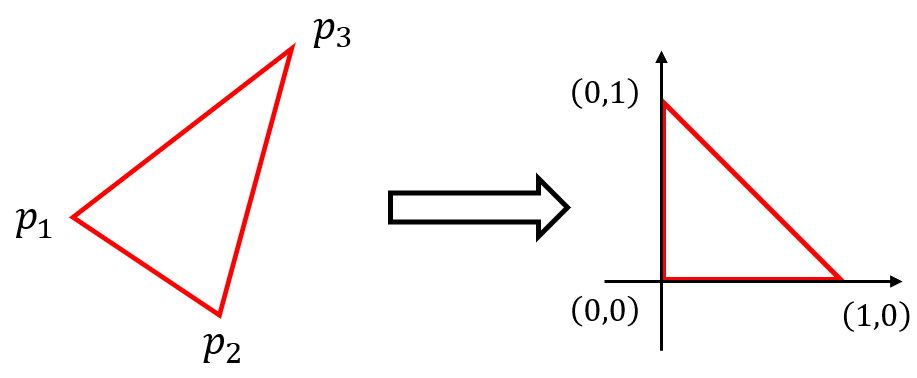
\includegraphics[width=0.4\textwidth]{./Figures/TriangleFromStandardTriangle.png}
    \caption{From triangle to standard triangle}
    \label{fig:tfst}
\end{figure}

From standard triangle $\left\{ {\left. {\left( {x,y} \right)} \right|0 \leqslant x,y \leqslant 1,x + y \leqslant 1} \right\}$ to stadard square $\left\{ {\left. {\left( {\xi ,\eta } \right)} \right| - 1 \leqslant \xi ,\eta  \leqslant 1} \right\}$

\begin{equation}
{s_k} = \frac{{1 + {\xi _i}}}{2},{t_k} = \frac{{\left( {1 - {\xi _i}} \right)\left( {1 + {\eta _j}} \right)}}{4},{c_k} = \frac{{\left( {1 - {\xi _i}} \right)}}{8}{w_i}{w_j},1 \leqslant k \leqslant {n^2},1 \leqslant i,j \leqslant n
\end{equation}
where $\xi _i, \eta _j$ and $w_i,w_j$ are Gauss points and weights, respectively.

\section{Contact}

\subsection{Global contact search}

$\rlap{$\checkmark$}\square$ \sout{The current bucket sort must satisfy: slave face is smaller than master face.}

\subsection{Local contact search}

master - non-mortar, slave - mortar;

\noindent $\blacksquare$ Project slave point onto master face

Point $\left[ {\bm{r}}_{\rm{s}} \right] = \left[ {\begin{array}{c} {r_{\rm{sx}}} \\ {r_{\rm{sy}}} \\ {r_{\rm{sz}}} \end{array}} \right]$ is on the slave face(segment), master face is given by

\begin{equation} \label{eq_rmxieta}
{{\bm{r}}_{\rm{m}}}\left( {\xi ,\eta } \right) = \sum\limits_{i = 1}^4 {{N_i}\left( {\xi ,\eta } \right){{\bm{r}}_{{\rm{m}}i}}}  = \left[ {\begin{array}{c}
  {{a_1} + {a_2}\xi  + {a_3}\eta  + {a_4}\xi \eta } \\ 
  {{b_1} + {b_2}\xi  + {b_3}\eta  + {b_4}\xi \eta } \\ 
  {{c_1} + {c_2}\xi  + {c_3}\eta  + {c_4}\xi \eta } 
\end{array}} \right]
\end{equation}

The tangential vector of master face is

\begin{equation} \label{eq_prmxiet}
\frac{{\partial {{\bm{r}}_{\rm{m}}}}}{{\partial \xi }} = \left[ {\begin{array}{c}
  {{a_2} + {a_4}\eta } \\ 
  {{b_2} + {b_4}\eta } \\ 
  {{c_2} + {c_4}\eta } 
\end{array}} \right],\frac{{\partial {{\bm{r}}_{\rm{m}}}}}{{\partial \eta }} = \left[ {\begin{array}{c}
  {{a_3} + {a_4}\xi } \\ 
  {{b_3} + {b_4}\xi } \\ 
  {{c_3} + {c_4}\xi } 
\end{array}} \right]
\end{equation}
\noindent\small * $\frac{{\partial {{\bm{r}}_{\rm{m}}}}}{{\partial \xi }}$ and $\frac{{\partial {{\bm{r}}_{\rm{m}}}}}{{\partial \eta }}$ are not perpendicular to each other.

The closest point projection implies

\begin{equation} \label{eq_closest}
\left\{ {\begin{array}{c}
  {\left( {{{\bm{r}}_{\rm{m}}}\left( {\xi ,\eta } \right) - {{\bm{r}}_{\rm{s}}}} \right) \cdot \frac{{\partial {{\bm{r}}_{\rm{m}}}\left( {\xi ,\eta } \right)}}{{\partial \xi }} = 0} \\ 
  {\left( {{{\bm{r}}_{\rm{m}}}\left( {\xi ,\eta } \right) - {{\bm{r}}_{\rm{s}}}} \right) \cdot \frac{{\partial {{\bm{r}}_{\rm{m}}}\left( {\xi ,\eta } \right)}}{{\partial \eta }} = 0} 
\end{array}} \right.
\end{equation}

After taking Eqs. (\ref{eq_rmxieta}) and (\ref{eq_prmxiet}) into Eq. (\ref{eq_closest}), the following 2-DOF nonlinear system of equations is obtained

\begin{equation}
\left\{ \begin{gathered}
  \left( {{a_1}{a_2} - {a_2}{r_{{\text{sx}}}} + {b_1}{b_2} - {b_2}{r_{{\text{sy}}}} + {c_1}{c_2} - {c_2}{r_{{\text{sz}}}}} \right) + \left( { + {a_2}{a_2} + {b_2}{b_2} + {c_2}{c_2}} \right)\xi  \hfill \\
   + \left( { + {a_2}{a_3} + {a_1}{a_4} - {a_4}{r_{{\text{sx}}}} + {b_2}{b_3} + {b_1}{b_4} - {b_4}{r_{{\text{sy}}}} + {c_2}{c_3} + {c_1}{c_4} - {c_4}{r_{{\text{sz}}}}} \right)\eta  \hfill \\
   + \left( { + 2{a_2}{a_4} + 2{b_2}{b_4} + 2{c_2}{c_4}} \right)\xi \eta  + \left( { + {a_3}{a_4} + {b_3}{b_4} + {c_3}{c_4}} \right){\eta ^2} + \left( { + {a_4}{a_4} + {b_4}{b_4} + {c_4}{c_4}} \right)\xi {\eta ^2} = 0 \hfill \\
  \left( {{a_1}{a_3} - {a_3}{r_{{\text{sx}}}} + {b_1}{b_3} - {b_3}{r_{{\text{sy}}}} + {c_1}{c_3} - {c_3}{r_{{\text{sz}}}}} \right) + \left( { + {a_3}{a_3} + {b_3}{b_3} + {c_3}{c_3}} \right)\eta  \hfill \\
   + \left( { + {a_2}{a_3} + {a_1}{a_4} - {a_4}{r_{{\text{sx}}}} + {b_2}{b_3} + {b_1}{b_4} - {b_4}{r_{{\text{sy}}}} + {c_2}{c_3} + {c_1}{c_4} - {c_4}{r_{{\text{sz}}}}} \right)\xi  \hfill \\
   + \left( { + 2{a_3}{a_4} + 2{b_3}{b_4} + 2{c_3}{c_4}} \right)\xi \eta  + \left( { + {a_2}{a_4} + {b_2}{b_4} + {c_2}{c_4}} \right){\xi ^2} + \left( { + {a_4}{a_4} + {b_4}{b_4} + {c_4}{c_4}} \right){\xi ^2}\eta  = 0 \hfill \\ 
\end{gathered}  \right.
\end{equation}

\noindent $\blacksquare$ Project master point back onto slave face

Point $\left[ {\bm{r}}_{\rm{m}} \right] = \left[ {\begin{array}{c} {r_{\rm{mx}}} \\ {r_{\rm{my}}} \\ {r_{\rm{mz}}} \end{array}} \right]$ is on the master face(segment), slave face is given by

\begin{equation} \label{eq_rsxieta}
{{\bm{r}}_{\rm{s}}}\left( {\xi ,\eta } \right) = \sum\limits_{i = 1}^4 {{N_i}\left( {\xi ,\eta } \right){{\bm{r}}_{{\rm{s}}i}}}  = \left[ {\begin{array}{c}
  {{a_1} + {a_2}\xi  + {a_3}\eta  + {a_4}\xi \eta } \\ 
  {{b_1} + {b_2}\xi  + {b_3}\eta  + {b_4}\xi \eta } \\ 
  {{c_1} + {c_2}\xi  + {c_3}\eta  + {c_4}\xi \eta } 
\end{array}} \right]
\end{equation}

The tangential vector of master face is

\begin{equation} \label{eq_prmxietM2S}
\frac{{\partial {{\bm{r}}_{\rm{m}}}}}{{\partial \xi }} = \left[ {\begin{array}{c}
  { r_{{\rm{m}} \xi x} } \\ 
  { r_{{\rm{m}} \xi y} } \\ 
  { r_{{\rm{m}} \xi z} } 
\end{array}} \right],\frac{{\partial {{\bm{r}}_{\rm{m}}}}}{{\partial \eta }} = \left[ {\begin{array}{c}
  { r_{{\rm{m}} \eta x} } \\ 
  { r_{{\rm{m}} \eta y} } \\ 
  { r_{{\rm{m}} \eta z} } 
\end{array}} \right]
\end{equation}

The closest point projection implies

\begin{equation} \label{eq_closestM2S}
\left\{ {\begin{array}{c}
  {\left( {{{\bm{r}}_{\rm{s}}} \left( {\xi ,\eta } \right)  - {{\bm{r}}_{\rm{m}}}} \right) \cdot \frac{{\partial {{\bm{r}}_{\rm{m}}} }}{{\partial \xi }} = 0} \\ 
  {\left( {{{\bm{r}}_{\rm{s}}} \left( {\xi ,\eta } \right)  - {{\bm{r}}_{\rm{m}}}} \right) \cdot \frac{{\partial {{\bm{r}}_{\rm{m}}} }}{{\partial \eta }} = 0} 
\end{array}} \right.
\end{equation}

After taking Eqs. (\ref{eq_rsxieta}) and (\ref{eq_prmxietM2S}) into Eq. (\ref{eq_closestM2S}), the following 2-DOF nonlinear system of equations is obtained

\begin{equation}
\left\{ \begin{gathered}
  \left( {{a_1}{r_{{\rm{m}}\xi x}} + {b_1}{r_{{\rm{m}}\xi y}} + {c_1}{r_{{\rm{m}}\xi z}} - {r_{\rm{m}}} \cdot \frac{{\partial {r_{\rm{m}}}}}{{\partial \xi }}} \right) + \left( {{a_2}{r_{{\rm{m}}\xi x}} + {b_2}{r_{{\rm{m}}\xi y}} + {c_2}{r_{{\rm{m}}\xi z}}} \right)\xi  \hfill \\
   + \left( {{a_3}{r_{{\rm{m}}\xi x}} + {b_3}{r_{{\rm{m}}\xi y}} + {c_3}{r_{{\rm{m}}\xi z}}} \right)\eta  + \left( {{a_4}{r_{{\rm{m}}\xi x}} + {b_4}{r_{{\rm{m}}\xi y}} + {c_4}{r_{{\rm{m}}\xi z}}} \right)\xi \eta  = 0 \hfill \\
  \left( { + {a_1}{r_{{\rm{m}}\eta x}} + {b_1}{r_{{\rm{m}}\eta y}} + {c_1}{r_{{\rm{m}}\eta z}} - {r_{\rm{m}}} \cdot \frac{{\partial {r_{\rm{m}}}}}{{\partial \eta }}} \right) + \left( {{a_2}{r_{{\rm{m}}\eta x}} + {b_2}{r_{{\rm{m}}\eta y}} + {c_2}{r_{{\rm{m}}\eta z}}} \right)\xi  \hfill \\
   + \left( {{a_3}{r_{{\rm{m}}\eta x}} + {b_3}{r_{{\rm{m}}\eta y}} + {c_3}{r_{{\rm{m}}\eta z}}} \right)\eta  + \left( {{a_4}{r_{{\rm{m}}\eta x}} + {b_4}{r_{{\rm{m}}\eta y}} + {c_4}{r_{{\rm{m}}\eta z}}} \right)\xi \eta  = 0 \hfill \\ 
\end{gathered}  \right.
\end{equation}

\noindent $\blacksquare$ Computational geometry

\begin{enumerate}[label=$\bullet$]
\item intersect of two 2d line segments;
\item calculating the area and centroid of a polygon in 2d \cite{PolygonCentroid};
\end{enumerate}

\section{Domain decomposition}

$\bigstar$ {\color{blue}{triangulation alignment for both ${\mathit{\Omega}}_H$ and ${\mathit{\Omega}}_h$.}}

\section{Linear algebra}

\subsection{Nonstationary solver}

\subsubsection{Conjugate gradient method}

\noindent $\blacksquare$ Semi-axis alignment \cite{Nocedal2006}: 

\begin{enumerate}[label=$\bullet$]
\item matrix ${{\bm{S}}^{\rm{T}}} {\bm{A}} {\bm{S}}$ is diagonal, 
${\bm{S}} = \left[ {{{\bm{p}}_0},{{\bm{p}}_1}, \cdots ,{{\bm{p}}_{n - 1}}} \right], {\bm{p}}_i^{\rm{T}} {\bm{A}} {{\bm{p}}_j} = 0,i \ne j$
\item coordinate transformation: $\hat {\bm{x}} = {{\bm{S}}^{ - 1}} {\bm{x}},\frac{1}{2} {\bm{x}} {\bm{A}} {\bm{x}} - { {\bm{b}} ^{\rm{T}}}{\bm{x}} = \frac{1}{2}\hat {\bm{x}}\left( {{ {\bm{S}} ^{\rm{T}}} {\bm{A}}  {\bm{S}} } \right)\hat {\bm{x}} - {\left( {{ {\bm{S}} ^{\rm{T}}} {\bm{b}} } \right)^{\rm{T}}}\hat x$
\item converges in $n$ iterations;
\end{enumerate}

\begin{figure}[htbp]
    \centering
    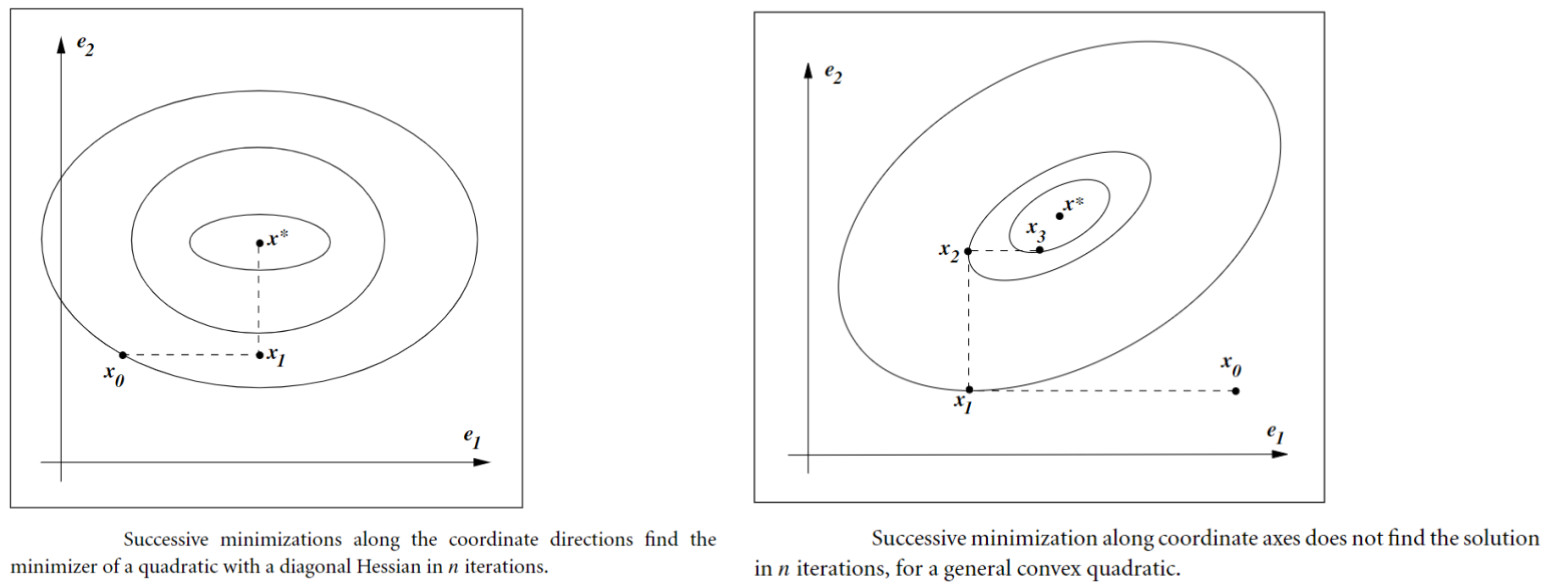
\includegraphics[width=0.95\textwidth]{./Figures/SemiAxisAlignment.jpg}
    \caption{Semi-axis alignment}
    \label{fig:semiaxisalignment}
\end{figure}

\noindent $\blacksquare$ Conjugate direction method

\begin{enumerate}[label=$\bullet$]
\item ${{\bm{x}}_{k + 1}} = {{\bm{x}}_k} + {\alpha _k}{{\bm{p}}_k}$. The step is determined by ``search direction is tangent to isoline'', $\alpha _k  = \frac{{ - {\bm{r}}_k^{\text{T}}{{\bm{p}}_k}}}{{{\bm{p}}_k^{\text{T}} {\bm{A}} {{\bm{p}}_k}}}$;
\begin{equation} \label{eq_rkp1rkkApk}
{{\bm{r}}_{k + 1}} = {{\bm{r}}_k} + {\alpha _k} {\bm{A}} {{\bm{p}}_k}
\end{equation}
\item In Fig.~\ref{fig:semiaxisalignment}, error ${{\bm{e}}_k} = {{\bm{x}}_k} - {{\bm{x}}^*}$ is conjugate to search direction ${\bm{e}}_k^{\text{T}} {\bm{A}} {\bm{p}_i} = 0,i = 0,1, \ldots ,k - 1$;
\item residual ${{\bm{r}}_k} = {\bm{A}} {{\bm{x}}_k} - b =  {\bm{A}} {{\bm{e}}_k}$ is orthogonal to search direction;
\begin{equation} \label{eq_rkTpi0}
{\bm{r}}_k^{\text{T}} {\bm{p}_i} = 0,i = 0,1, \ldots ,k - 1
\end{equation}
\end{enumerate}

\noindent $\blacksquare$ Conjugate gradient method \cite{Shewchuk1994} Fig.~\ref{fig:ConjugateGradient}

\begin{figure}[htbp]
    \centering
    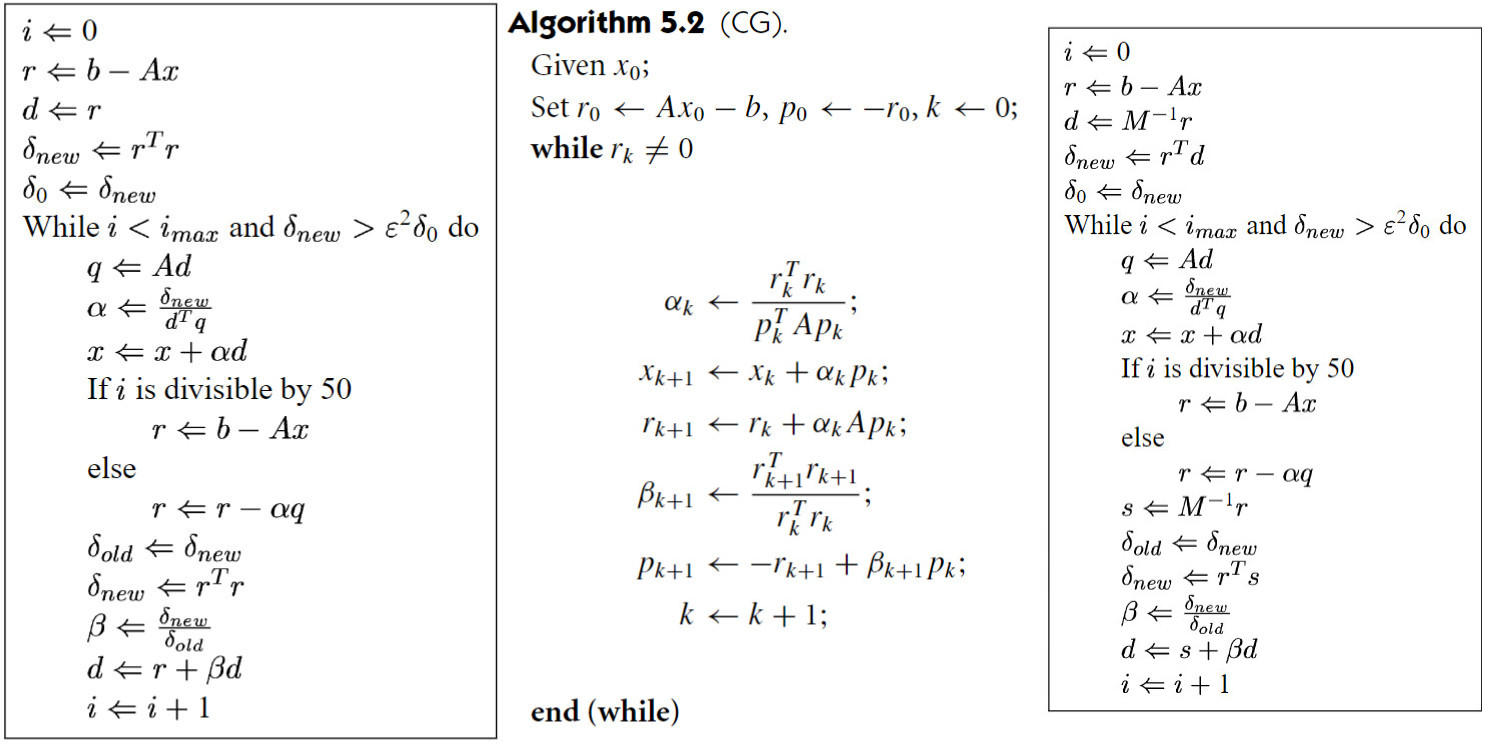
\includegraphics[width=0.8\textwidth]{./Figures/ConjugateGradient.jpg}
    \caption{Conjugate gradient method}
    \label{fig:ConjugateGradient}
\end{figure}

\begin{enumerate}[label=$\bullet$]
\item select search direction by gradient 
\begin{equation} \label{eq_pkrkkpk}
{{\bm{p}}_0} = {{\bm{r}}_0}, {{\bm{p}}_k} =  - {{\bm{r}}_k} + {\beta _k}{{\bm{p}}_{k - 1}}
\end{equation}
\item the coefficient is determined by ``${{\bm{p}}_k}$ and ${{\bm{p}}_{k-1}}$ are conjugate'', ${\beta _k} = \frac{{{\bm{r}}_k^{\text{T}} {\bm{A}} {{\bm{p}}_{k - 1}}}}{{{\bm{p}}_{k - 1}^{\text{T}} {\bm{A}} {{\bm{p}}_{k - 1}}}}$;
\item From Eqs.~(\ref{eq_rkp1rkkApk}) and (\ref{eq_pkrkkpk}), the Krylov space
\begin{equation} \label{eq_spanrkkpk}
\operatorname{span} \left\{ {{{\bm{r}}_0},{{\bm{r}}_1}, \ldots ,{{\bm{r}}_k}} \right\} = \operatorname{span} \left\{ {{{\bm{p}}_0},{{\bm{p}}_1}, \ldots ,{{\bm{p}}_k}} \right\}  = \operatorname{span} \left\{ {{{\bm{r}}_0},{\bm{A}}{{\bm{r}}_0}, \ldots ,{{\bm{A}}^k}{{\bm{r}}_0}} \right\}
\end{equation}
\item From Eqs.~(\ref{eq_rkTpi0}) and (\ref{eq_spanrkkpk}), residuals are orthogonal to each other ${\bm{r}}_k^{\text{T}} {{\bm{r}}_i} = 0,i = 0,1, \ldots ,k - 1$;
\item Search directions are conjugate to each other ${\bm{p}}_k^{\text{T}} {\bm{A}} {{\bm{p}}_i} = 0,i = 0,1, \ldots ,k - 1$. $A{p_{i-2}} \subset \operatorname{span} \left\{ {{{\bm{r}}_0},{{\bm{r}}_1}, \ldots ,{{\bm{r}}_{i-1}}} \right\}$
\item Simplification: from Eq.~(\ref{eq_rkp1rkkApk}), ${\alpha _k} = \frac{{ {\bm{r}}_k^{\text{T}}{ {\bm{r}}_k}}}{{ {\bm{p}}_k^{\text{T}} {\bm{A}} { {\bm{p}}_k}}}$; from Eqs.~(\ref{eq_rkp1rkkApk}) and (\ref{eq_pkrkkpk}), ${\beta _{k + 1}} = \frac{{ {\bm{r}}_{k + 1}^{\text{T}}{ {\bm{r}}_{k + 1}}}}{{ {\bm{r}}_k^{\text{T}}{ {\bm{r}}_k}}}$
\end{enumerate}

\subsubsection{Chebyshev polynomial}

\noindent $\blacksquare$ Why Chebyshev polynomial

\begin{figure}[htbp]
    \centering
    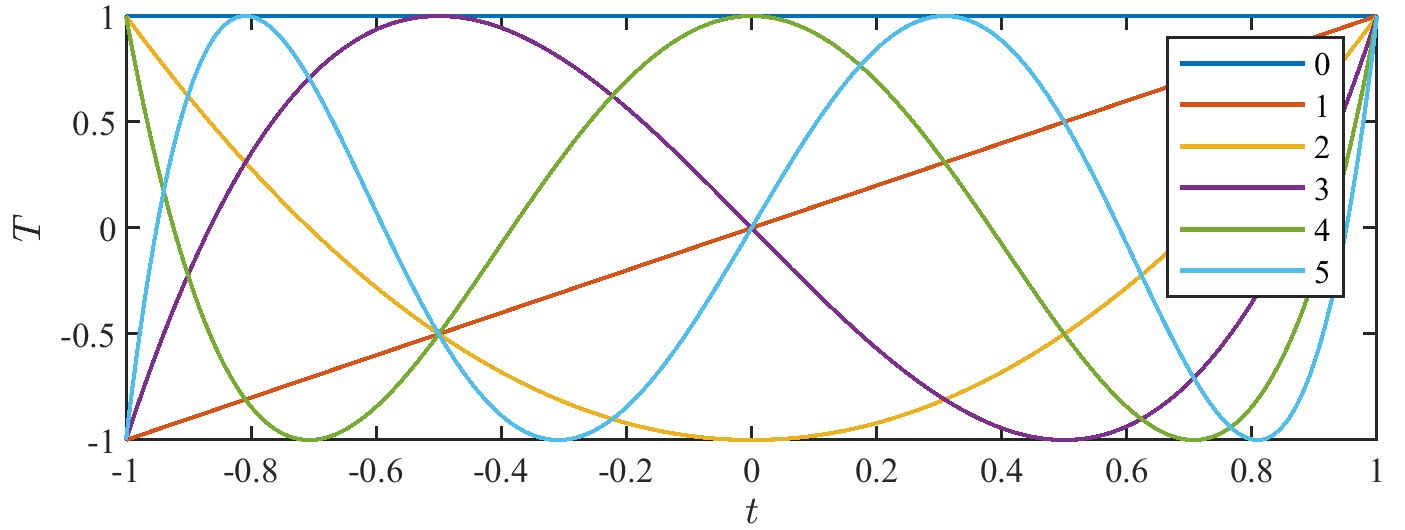
\includegraphics[width=0.6\textwidth]{./Figures/Chebyshev.jpg}
    \caption{Chebyshev polynomial}
    \label{fig:Chebyshev}
\end{figure}

\begin{enumerate}[label=$\bullet$]
\item Chebyshev polynomial
\begin{equation}
{T_0}\left( t \right) = 1,{T_1}\left( t \right) = t,{T_k}\left( t \right) = 2t{T_{k - 1}}\left( t \right) - {T_{k - 2}}\left( t \right)
\end{equation}
\begin{equation}
d = \frac{{{\lambda _{\max }} + {\lambda _{\min }}}}{2},c = \frac{{{\lambda _{\max }} - {\lambda _{\min }}}}{2},t = \frac{{\lambda  - d}}{c}, 0 < {\lambda _{\min }} \leqslant \lambda  \leqslant {\lambda _{\max }} <  + \infty 
\end{equation}
\begin{equation}
{\bm{A}} = {\bm{Q}}{\bm{\Lambda}} {{\bm{Q}}^{\rm{T}}},\frac{{{\bm{A}} - d{\bf{I}}}}{c} = {\bm{Q}}\frac{{{\bm{\Lambda}}  - d{\bf{I}}}}{c}{{\bm{Q}}^{\rm{T}}},{T_k}\left( {\frac{{{\bm{A}} - d{\bf{I}}}}{c}} \right) = {\bm{Q}} {T_k}\left( {\frac{{{\bm{\Lambda}}  - d{\bf{I}}}}{c}} \right){{\bm{Q}}^{\rm{T}}}
\end{equation}
\item The smaller $P \left( \lambda _i \right)$ is, the better: Chebyshev polynomial $\left| {{T_k}\left( t \right)} \right| \leqslant 1, - 1 \leqslant t \leqslant 1$ is a good choice.
\begin{equation}
{{\bm{e}}_0} = {{\bm{x}}^*} - {{\bm{x}}_0} = {\bm{Q}}{{\bm{\xi}} _0}, P\left( {\bm{A}} \right){{\bm{e}}_0} = {\bm{Q}}P\left( {\bm{\Lambda}}  \right){{\bm{Q}}^T}{\bm{Q}}{{\bm{\xi}} _0} = {\bm{Q}}P\left( {\bm{\Lambda}}  \right){{\bm{\xi}} _0}
\end{equation}
\end{enumerate}

\noindent $\blacksquare$ Chebyshev iteration

\begin{equation} \label{eq_chebyshev}
\left\{ {\begin{array}{c}
  {{{\bm{r}}_k} = {\bm{b}} - {\bm{A}}{{\bm{x}}_k}} \\ 
  {{{\bm{p}}_k} = {\alpha _k}{{\bm{r}}_k} + {\beta _k}{{\bm{p}}_{k - 1}}, {\bm{p}}_{-1} = {\bm{0}}} \\ 
  {{{\bm{x}}_{k + 1}} = {{\bm{x}}_k} + {{\bm{p}}_k}} 
\end{array}} \right.
\end{equation}

\begin{enumerate}[label=$\bullet$]
\item From ${{\bm{r}}_k} = {\bm{A}}{{\bm{e}}_k}$ and the second equation of Eq.~(\ref{eq_chebyshev}), search direction
\begin{equation}
{{\bm{p}}_k} = \left[ {{\bf{I}} - {P_{k + 1}}\left( {\bm{A}} \right)} \right]{{\bm{e}}_0}
\end{equation}
\item Error update = error multiplied by polynomial
\begin{equation}
{{\bm{e}}_{k + 1}} = {{\bm{x}}^*} - {{\bm{x}}_{k + 1}} = {{\bm{e}}_k} - {{\bm{p}}_k} = {P_{k + 1}}\left( {\bm{A}} \right){{\bm{e}}_0}
\end{equation}
\begin{equation}
{{\bm{e}}_1} = \left( {{\bf{I}} - \frac{1}{d}{\bm{A}}} \right){{\bm{e}}_0}, 
{P_1}\left( {{\lambda _i}} \right) = 1 - \frac{{{\lambda _i}}}{d} =  - \frac{c}{d}{T_1}\left( {\frac{{{\lambda _i} - d}}{c}} \right)
\end{equation}
\begin{equation}
{e_2} = \left( {{\bf{I}} - \frac{2}{d}{\bm{A}} + \frac{{2{{\bm{A}}^2}}}{{2{d^2} - {c^2}}}} \right){{\bm{e}}_0},{P_2}\left( {{\lambda _i}} \right) = 1 - \frac{{2{\lambda _i}}}{d} + \frac{{2\lambda _i^2}}{{2{d^2} - {c^2}}} = {T_2}\left( {\frac{{{\lambda _i} - d}}{c}} \right)
\end{equation}
\item According to that ${P_{k + 1}}\left( {\bm{A}} \right)$ is Chebyshev polynomial, coefficients $\alpha _k$ and $\beta _k$ can be determined. The above actually gives a verification for this.
\begin{equation}
{\alpha _0} = \frac{1}{d},{\beta _0} = 0;{\alpha _1} = \frac{{2d}}{{2{d^2} - {c^2}}},{\beta _1} = {\alpha _1}d - 1;{\alpha _k} = \frac{1}{{d - \frac{{{c^2}}}{4}{\alpha _{k - 1}}}},{\beta _k} = {\alpha _k}d - 1
\end{equation}
\end{enumerate}

\subsection{Stationary solver}

\begin{enumerate}[label=$\blacksquare$]
\item Matrix partitioning ${\bm{A}} = {\bm{D}} + {\bm{L}} + {\bm{U}}$;
\item Jacobian ${{\bm{x}}^{\left( {k + 1} \right)}} = {{\bm{D}}^{ - 1}}\left[ {{\bm{b}} - \left( {\bm{L}} + {\bm{U}} \right) {{\bm{x}}^{\left( k \right)}}} \right]$;
\item Gauss-Seidel ${{\bm{x}}^{\left( {k + 1} \right)}} = {{\bm{D}}^{ - 1}}\left( {{\bm{b}} - {\bm{L}}{{\bm{x}}^{\left( {k + 1} \right)}} - {\bm{U}}{{\bm{x}}^{\left( k \right)}}} \right)$;
  \begin{enumerate}[label=$\bullet$]
  \item ${{\bm{x}}^{\left( {k + 1} \right)}} = {\left( {{\bm{D}} + {\bm{L}}} \right)^{ - 1}}\left( { {\bm{b}} - {\bm{U}}  {{\bm{x}}^{\left( k \right)}}} \right)$;
  \end{enumerate}
\item Symmetric Gauss-Seidel
  \begin{enumerate}[label=$\bullet$]
  \item ${{\bm{x}}_1} = {\left( {{\bm{D}} + {\bm{L}}} \right)^{ - 1}}\left( { {\bm{b}} - {\bm{U}}  {{\bm{x}}_0}} \right)$;
  \item ${{\bm{x}}_2} = {\left( {{\bm{D}} + {\bm{U}}} \right)^{ - 1}}\left( { {\bm{b}} - {\bm{L}}  {{\bm{x}}_1}} \right)  = {\left( {{\bm{D}} + {\bm{U}}} \right)^{ - 1}}\left( {{\bm{D}}{{\bm{x}}_1} + {\bm{U}}{{\bm{x}}_0}} \right)$ reuses ${\bm{U}}{{\bm{x}}_0}$;
  \end{enumerate}
\item Successive over-relaxation (SOR) ${{\bm{x}}^{\left( {k + 1} \right)}} = \left( {1 - \omega } \right){{\bm{x}}^{\left( k \right)}} + \omega {{\bm{D}}^{ - 1}}\left( {{\bm{b}} - {\bm{L}}{{\bm{x}}^{\left( {k + 1} \right)}} - {\bm{U}}{{\bm{x}}^{\left( k \right)}}} \right)$;
  \begin{enumerate}[label=$\bullet$]
  \item ${{\bm{x}}^{\left( {k + 1} \right)}} = {\left( {{\bm{D}} + \omega {\bm{L}}} \right)^{ - 1}} \left\{ \left[ {\left( {1 - \omega } \right){\bm{D}} - \omega {\bm{U}}} \right]{{\bm{x}}^{\left( k \right)}} + \omega {\bm{b}} \right\}$;
  \end{enumerate}
\item Symmetric SOR (SSOR)
  \begin{enumerate}[label=$\bullet$]
  \item ${{\bm{x}}_1} = {\left( {{\bm{D}} + \omega {\bm{L}}} \right)^{ - 1}}\left[ {\left( {1 - \omega } \right){\bm{D}} - \omega {\bm{U}}} \right]{{\bm{x}}_0} + \omega {\left( {{\bm{D}} + \omega {\bm{L}}} \right)^{ - 1}}{\bm{b}} = {\left( {{\bm{D}} + \omega {\bm{L}}} \right)^{ - 1}} \left( {\bm{p}}_0 + \omega {\bm{b}} \right)$;
  \item ${{\bm{x}}_2} = {\left( {{\bm{D}} + \omega {\bm{U}}} \right)^{ - 1}}\left[ {\left( {1 - \omega } \right){\bm{D}} - \omega {\bm{L}}} \right]{{\bm{x}}_1} + \omega {\left( {{\bm{D}} + \omega {\bm{U}}} \right)^{ - 1}}{\bm{b}} = {\left( {{\bm{D}} + \omega {\bm{U}}} \right)^{ - 1}}\left[ {\left( {2 - \omega } \right){\bm{D}} {{\bm{x}}_1} - {{\bm{p}}_0} } \right]$;
  \end{enumerate}
\end{enumerate}

\subsection{Multigrid method}

\begin{figure}[htbp]
    \centering
    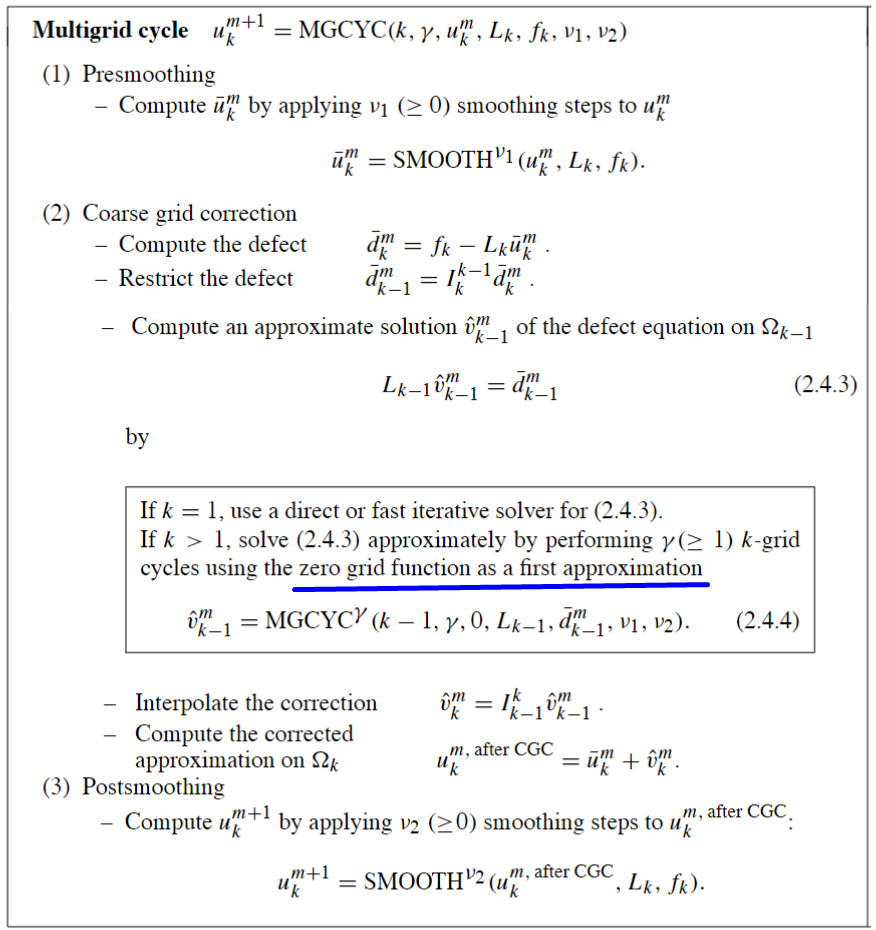
\includegraphics[width=0.6\textwidth]{./Figures/Multigrid.jpg}
    \caption{Multigrid method \cite{Trottenberg2001}}
    \label{fig:multigrid}
\end{figure}

\section{Computer science}

\subsection{Hardware}

\subsubsection{CPU}

\begin{figure}[htbp]
    \centering
    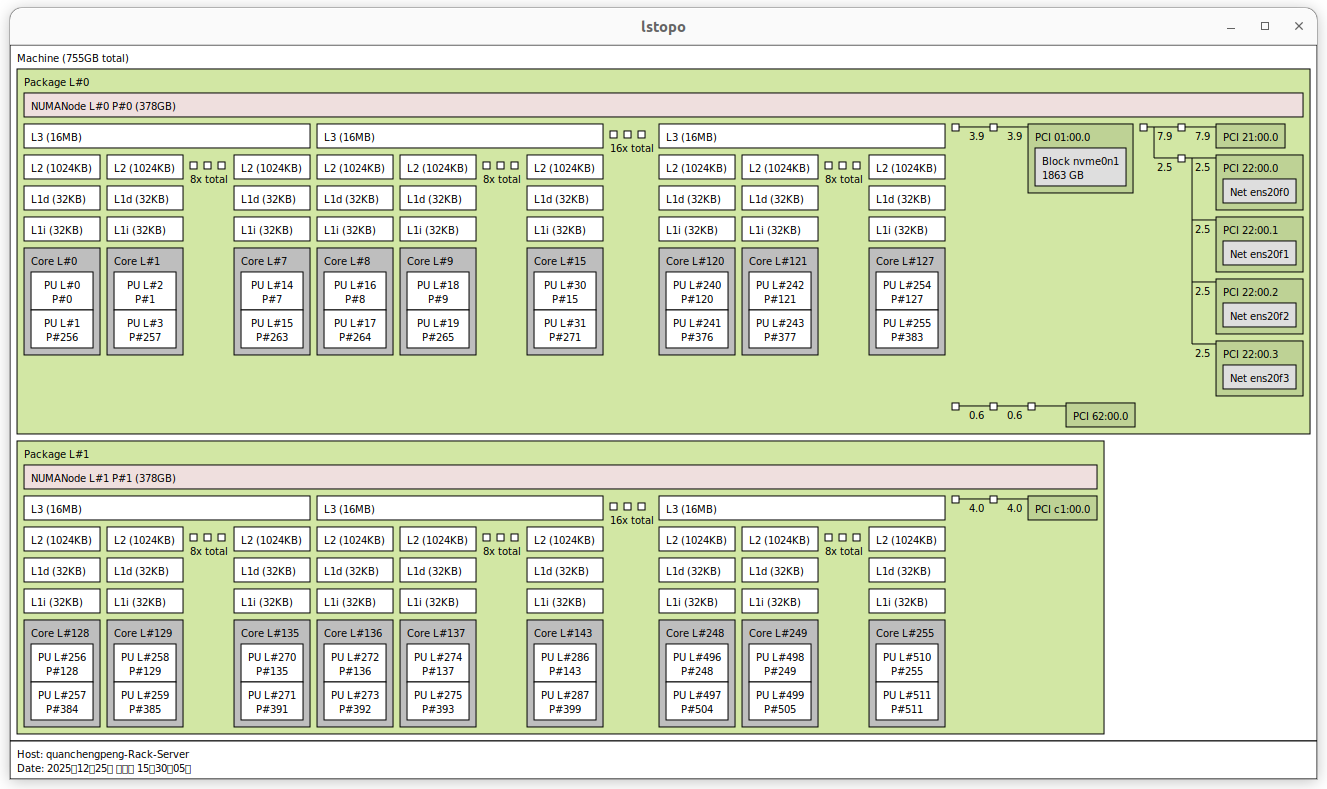
\includegraphics[width=1.0\textwidth]{./Figures/lstopo.png}
    \caption{lstopo}
    \label{fig:lstopo} % 标签，用于交叉引用
\end{figure}

\begin{enumerate}[label=$\blacksquare$]
\item Caching
  \begin{enumerate}[label=$\bullet$]
  \item Every CPU core has its own L1/L2 caching, all CPU cores share L3 caching; 
  \item TLB: from virtual address to real phsical address. Every CPU core has its own L1/L2 DTLB, all CPU cores share L3 DTLB;
  \end{enumerate}
\item NUMA (Non-Uniform Memory Access)
  \begin{enumerate}[label=$\bullet$]
  \item Different to SMP;
  \item Every NUMA node has its own CPU cores and local memory;
  \item For a CPU core in NUMA node 1, the latency to access local memory is much lower than that to access the remote memory (local memory of NUMA node 2);
  \end{enumerate}
\end{enumerate}

\subsubsection{Interface}

\begin{figure}[htbp]
    \centering
    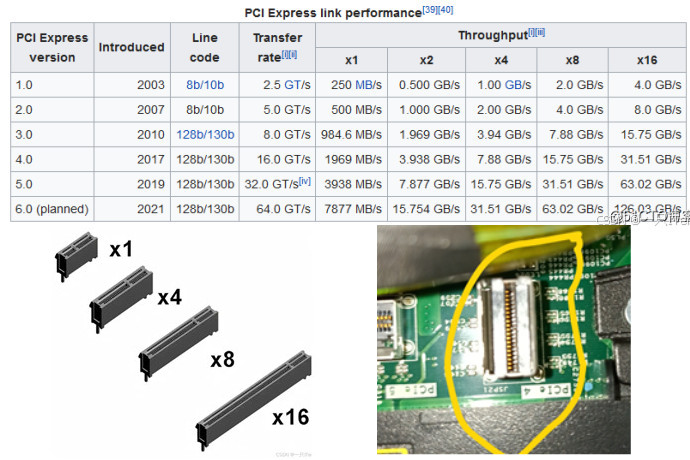
\includegraphics[width=0.9\textwidth]{./Figures/PCIe.jpg}
    \caption{PCIe}
    \label{fig:PCIe}
\end{figure}

\begin{figure}[htbp]
    \centering
    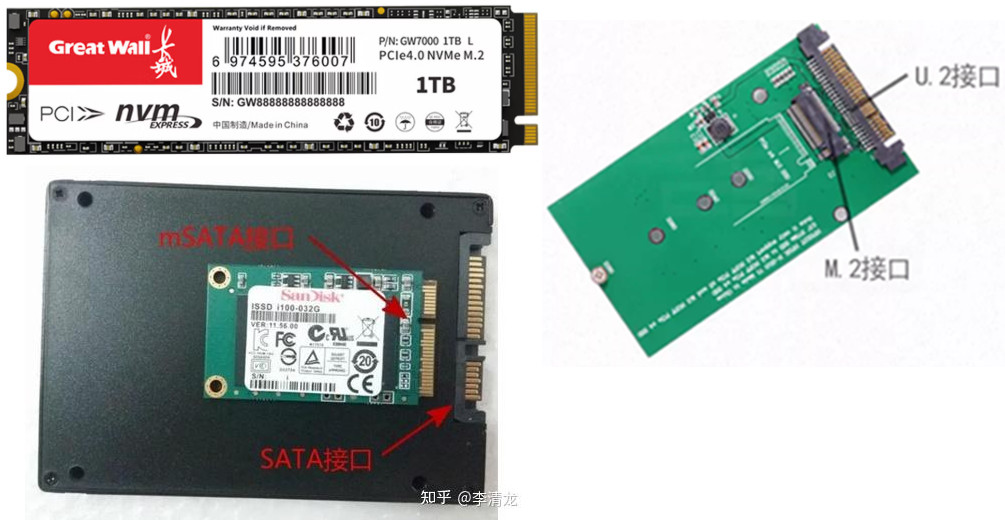
\includegraphics[width=0.8\textwidth]{./Figures/M.2U.2SATA.jpg}
    \caption{M.2, U.2, SATA}
    \label{fig:M2U2SATA}
\end{figure}

\begin{enumerate}[label=$\blacksquare$]
\item PCIe Fig.~\ref{fig:PCIe}
  \begin{enumerate}[label=$\bullet$]
  \item PCIE x1, x4, x8, x16, 1.0, 2.0, 3.0, 4.0, 5.0;
  \item PCIe Mini SAS HD;
  \end{enumerate}
\item Hard disk
  \begin{enumerate}[label=$\bullet$]
  \item U.2 (NVME PCIe), M.2 (NVME PCIe), SATA Fig.~\ref{fig:M2U2SATA};
  \end{enumerate}
\end{enumerate}

\subsection{Software}

\begin{enumerate}[label=$\blacksquare$]
\item Plain old data
\item \lstinline{semaphore} is much more stable than \lstinline{condition_variable};
\item Even if the output is right, we can not say that the code is right: there must be always bugs!
\end{enumerate}

\subsection{Architecture}

\begin{enumerate}[label=$\blacksquare$]
\item Distributed parallelism
  \begin{enumerate}[label=$\bullet$]
  \item Mater node, workder node: the same operating system (all Ubuntu 22.04.5LTS), the same LAN, the same hostname resolution /etc/hosts, the same username;
  \item SSH no password;
  \item hostfile on master node; Slurm --with-slurm;
  \end{enumerate}
\end{enumerate}

\section{Miscellaneous}

\subsection{Important}

\begin{enumerate}[label=$\blacksquare$]
\item \lstinline{GeometricMultigrid.cpp}: the level difference of two adjcent elements $<= 1$;
\end{enumerate}

\subsection{Moderate}

\begin{enumerate}[label=$\blacksquare$]
\item Thread management parameters
  \begin{enumerate}[label=$\bullet$]
  \item Preferably, \lstinline{numbThreads} is divisible by \lstinline{threadsPerDomain/threadsPerInterface};
  \item Total number of levels: \lstinline{maxLevel + 2}, \lstinline{0 ~ maxLevel + 1};
  \item By default, the AMD SMT is enabled;
  \end{enumerate}
\item \lstinline{Log} is not thread safe: better performance;
\item \lstinline{pthread.h}: only support Ubuntu;
\item At most two levels of nested parallelism;
\item The nested parallelism in \lstinline{GeometricMultigrid.cpp} is much more complicated!!!!!
\end{enumerate}

\section{Prospect}

\begin{enumerate}[label=$\blacksquare$]
\item add RAM, see can it less than 100s: very sure it can when the 24 memory slots are all used!
\item learn distributed parallelism with openMPI: try the scnet;
\item why abandon "nested parallelism":
  \begin{enumerate}[label=$\bullet$]
  \item pursuit for scalability: one CPU core for one domain will be the best choice (or at least a closing choice); Otherwise, how to explain the reason that nested parallelism is better than "one CPU core for one domain";
  \item openMPI will be much better in order to avoid access conflict of L3 cache;
  \end{enumerate}
\item Self-establish is too expensive: i3-12100f 4C 3.4GHz, 500 * 256 = 128000; ddr5 16G, 500 * 256 = 128000;
\item Self-establish: E8400 2C 3.0GHz+G45 motherboard, 161 * 128 = 20608; ddr3 8G, 100 * 128 = 12800; 128G SSD, 90*128 = 11520; 
\item What is the difference: interpolation of displacement and then projected onto normal direction; interpolation of normal displacement;
\end{enumerate}

\bibliographystyle{unsrt}
\bibliography{References}